Models of particle dark matter involving SM-DM interactions necessarily link searches for DM at collider and searches in direct and direct detection experiments. Figures~\ref{fig:Complementarity} (a-c) show that, in the EFT paradigm, different search strategies are simply looking at the same process from different perspectives: DM can interact in the lab in DD experiments, it can be observed in space %galaxies is too close to snowmass formulation "indirect detection experiments that connect lab signals to dark matter in our own and other galaxies"
by ID experiments, and it can be created in the lab by colliders and observed by experiments such as ATLAS, CMS and LHCb. This complementarity of multiple search targets in different experiments is necessary to elucidate the nature of dark matter in case of a discovery. Collider experiments are unable to determine whether a new phenomenon with the signatures discussed in Sec.~\ref{sec:03_ExperimentalResults}, originates from an invisible particle or from a DM mediator. 
%Good sentence from DMF 
%One advantage of collider experiments lies in their ability to study and possibly characterize the mediator. A discovery of an anomalous E/T signature at the LHC would not uniquely imply discovery of dark matter, while at the same time e.g. discovery of an anomalous and annually-modulated signal in a direct-detection experiment would leave unanswered many questions about the nature of the interaction that could be resolved by the simultaneous discovery of a new mediator particle. Collider, direct, and indirect detection searches provide complementary ways to approach this problem [50], and it is in this spirit that much of our focus is on the mediator.

On the other hand, collider experiment can make a prediction for the signal strength of a particular model and test its consistency with relic density. This prediction can be verified in presence of a signal in DD and ID, and the connection with the galactic nature of the new phenomenon can be established. Colliders can also shed light on the physics processes that complement DM production, e.g. as in Fig.~\ref{fig:Complementarity} (d) colliders can discover the new particle mediating the interaction and measure its coupling to SM particles other than quarks and gluons. %would be nice to give some literature here but no space

%Note on this figure: it's on wikimedia before i submitted the nature physics because I planned to reuse it here and told nature physics i wanted it cited but nature physics being the predatory shit paper that it is ignored all my request of creative commons (but they redid it with thinner lines). maybe we reword the caption?
\begin{figure}[!htpb]
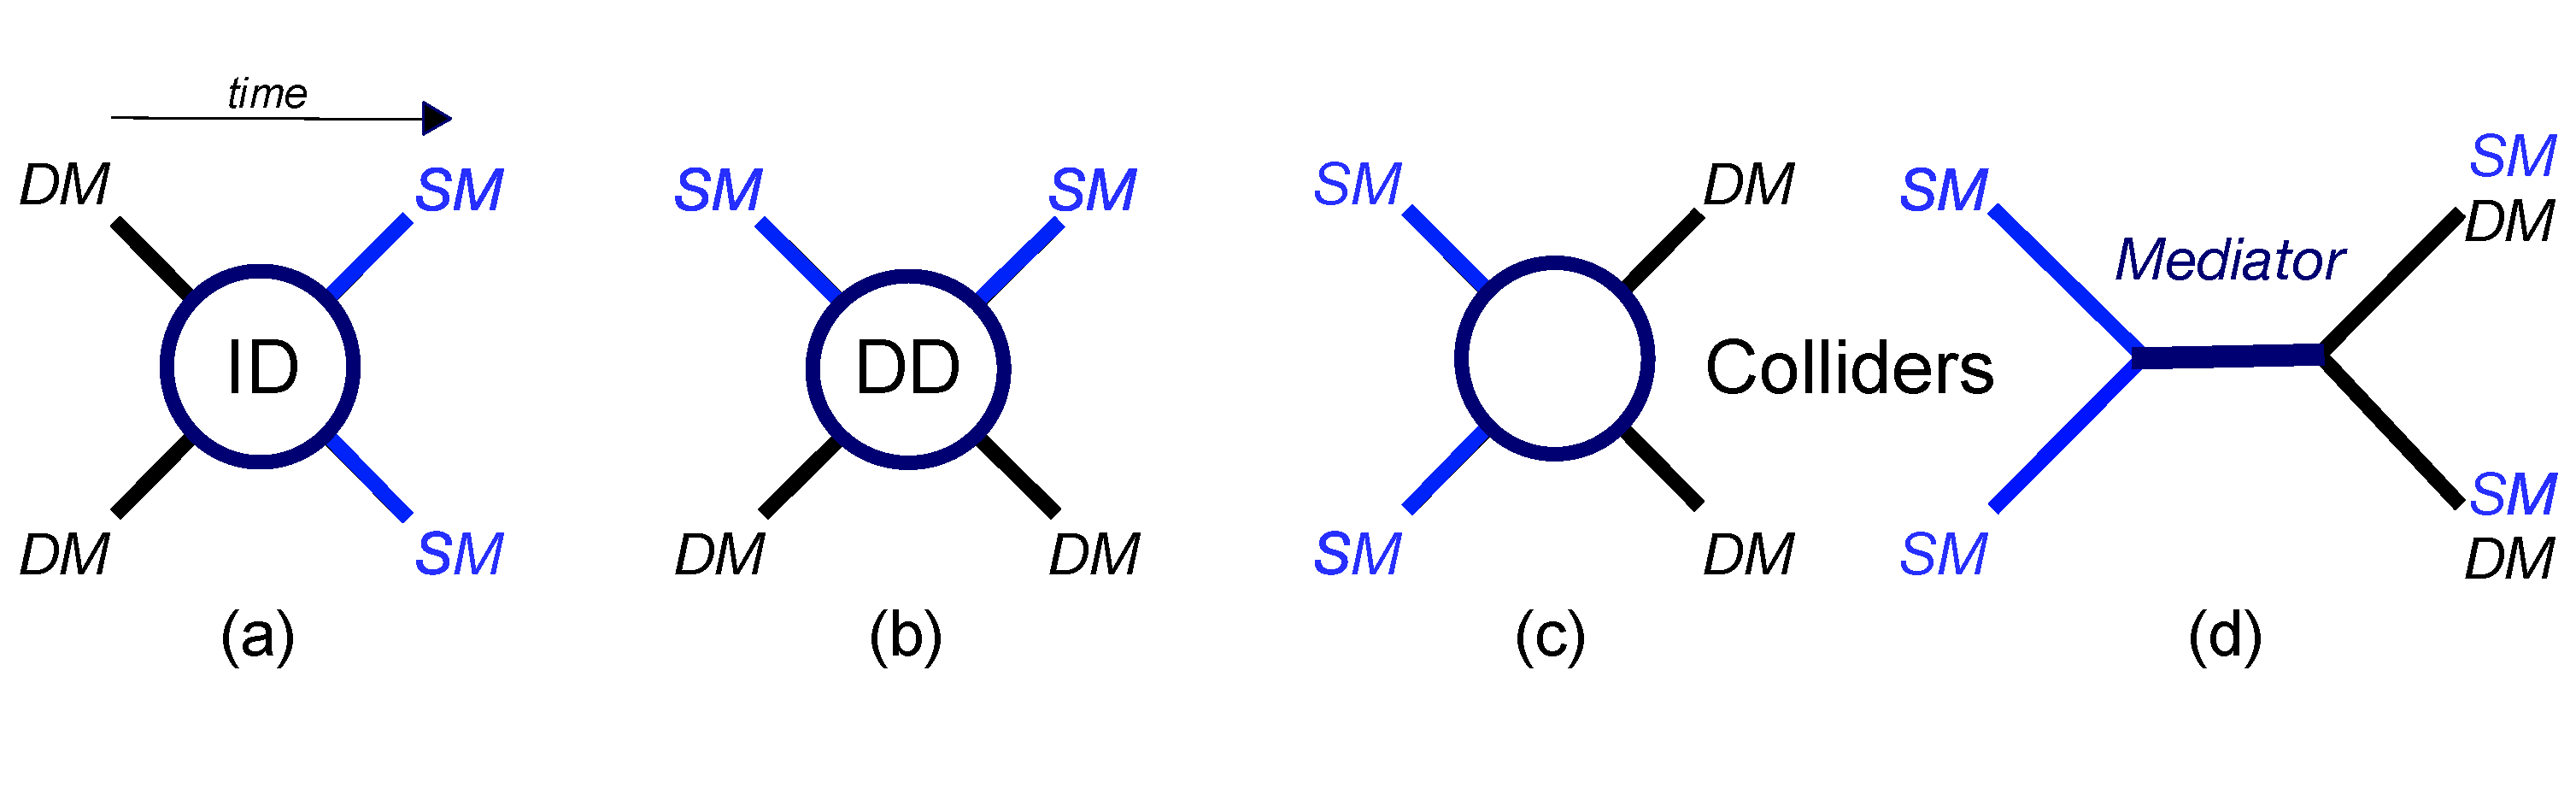
\includegraphics[width=\textwidth]{figures/EFTSimplifiedModels}
\caption{Schematic illustration of Dark Matter interactions and their corresponding experimental detection techniques, with time flowing from left to right. Fig. (a) shows DM annihilation to Standard Model particles, as sought by Indirect Detection (ID) experiments. Fig. (b) shows DM -> SM particle scattering, targeted by Direct Detection (DD) experiments. Fig. (c) shows the production of DM particles from the annihilation of SM particles at colliders. Fig. (d) shows again the pair production of DM at colliders as in (c), but in this case the interaction occurs through a mediator particle between DM and SM particles. From~\cite{monoXfig}, inspired by ~\cite{Bauer:2013ihz}.}
\label{fig:Complementarity}
\end{figure}

It is also worth mentioning that, even though comparisons between collider, DD and ID have become, the comparison with
LHC, DD and ID results with results from astrophysics is a growing field. 
This is particularly important since all the observational evidence of DM that we have is gravitational,
so DM properties such as mass and density in our and other galaxies
can be inferred from galaxy simulations or deviations in astrophysical observables, 
and signatures of DM self-interactions in rotation galaxies or cluster collisions can complement and verify any DD 
observations. Even though we do not cover this topic in detail in this review we refer to~\cite{Buckley:2017ijx}. 

\subsection{Comparing LHC constraints from visible and invisible searches with non-collider results}

The comparison of results from complementary experiments needs a mechanism to relate the processes
that will produce a signal in each type of detectors. This ultimately means that any comparison between LHC, DD and ID
needs a fully specified theoretical benchmark to be predictive and consistent. Since there are a large possible number of options to choose from, it is always important to keep in mind that such comparisons are model-dependent and the choice of benchmark can have severe implications for the conclusions drawn. 

%%LHC -> DD/ID

%EFT
Tevatron and Run-1 LHC searches mainly used EFTs as the common theoretical ground to compare their constraints on DM across experiments, or full models such as SUSY. EFTs are a good and flexible benchmark model to represent DM interactions in DD and ID experiment, since the momentum transfer of the collision is sufficiently low not to resolve the theory beyond the scale of the interaction and certainly below the electroweak scale. As discussed in Sec.~\ref{sub:EFT}, this is not always the case for high-energy collider experiments. The difference in interaction scales also requires that any operator in the model is evolved from the scale of the LHC collisions to the nuclear scale of DD through renormalization group expansion (RGE)~\cite{DEramo:2014nmf} for full consistency of the results. %is it clear enough that this has to be done for simplified models too? 
An example of a comparison plot between collider and DD results using EFT operators in the WIMP-nucleon cross-section vs WIMP mass plane\footnote{The formulas to translate LHC limits to this plane can be found in Ref.~\cite{Goodman:2010ku}}, without evolving the operators using RGE but showing the effects of the truncation of the events where the EFT is invalid, is shown for the LHC Run-1 results in Fig.~\ref{fig:SIATLASEFT}. %There isn't enough space to describe the results of the truncation in detail
What can be inferred from the plot is that within this class of models and spin assumption %We could have a footnote on SD and SI but no room in text?
the ideal region for the discovery of DM is that where WIMPs have masses above 10 GeV, as both collider and DD experiments are sensitive and could verify each other's claims. Next-generation DD experiments are expected to lower the minimum sensitivity thresholds in the next decade, see e.g.~\cite{Agnese:2016cpb}. 

\begin{figure}[!htpb]
%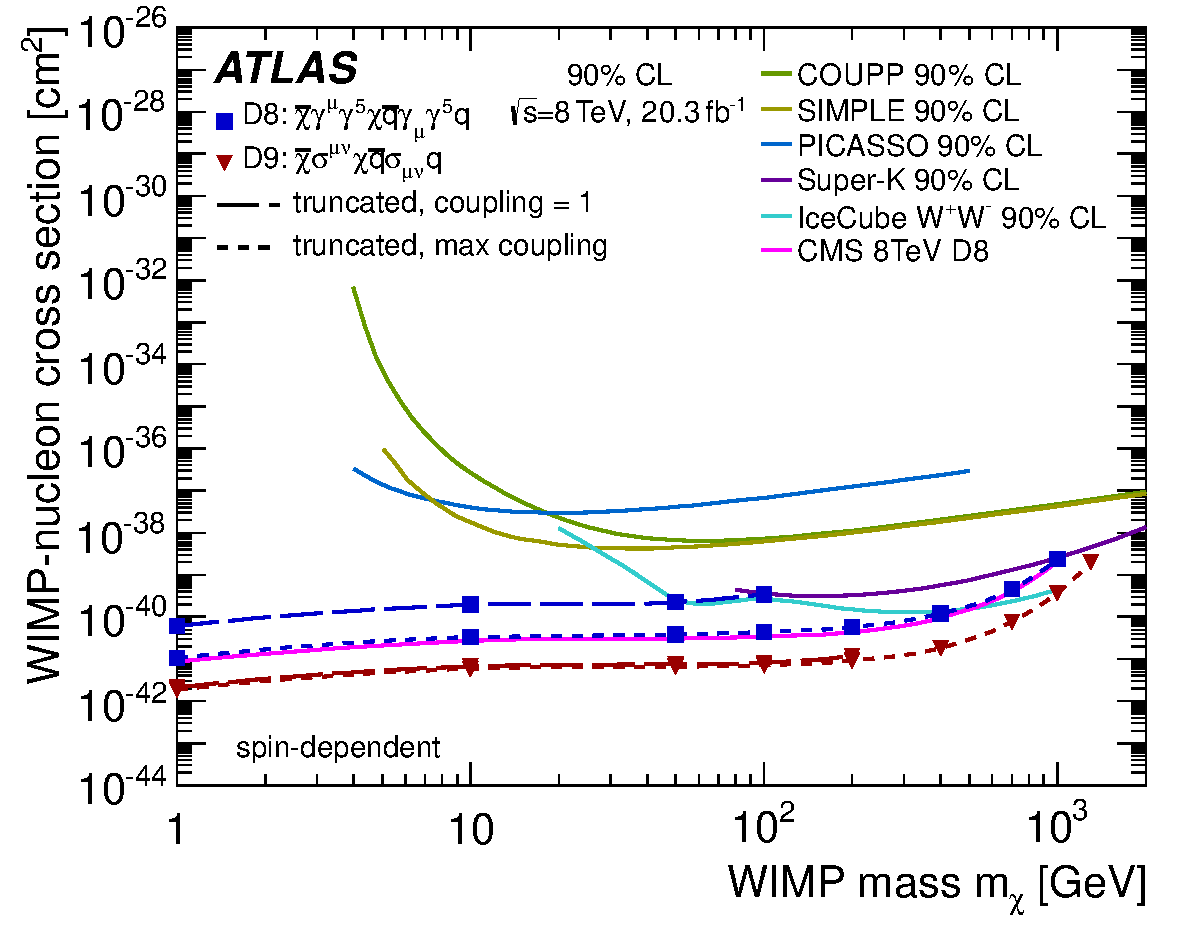
\includegraphics[width=0.35\textwidth]{figures/Monojet8TeV_EFT_SD}
%Can't have both so choose less controversial
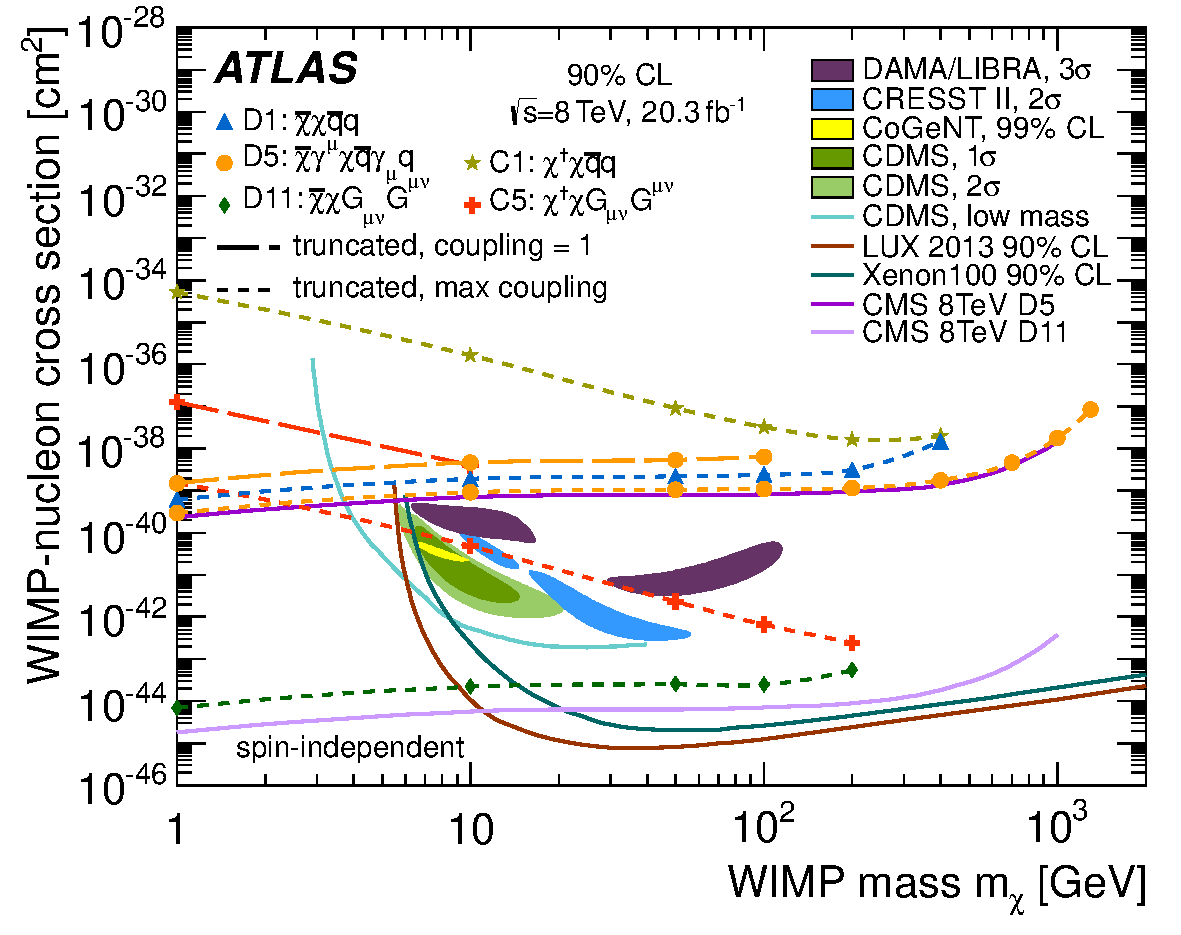
\includegraphics[width=0.9\textwidth]{figures/Monojet8TeV_EFT_SI}
\caption{Inferred 90\% CL limits on (left) the spin-independent and (right) spin-dependent WIMP--nucleon scattering cross section as a function of DM mass m? for different operators. Results from direct-detection experiments for the spin-independent and spin-dependent cross section, and the CMS (untruncated) results are shown for comparison. From~\cite{monoXfig}.}
\label{fig:SIATLASEFT}
\end{figure}

%Simp

\begin{figure}[!htpb]
%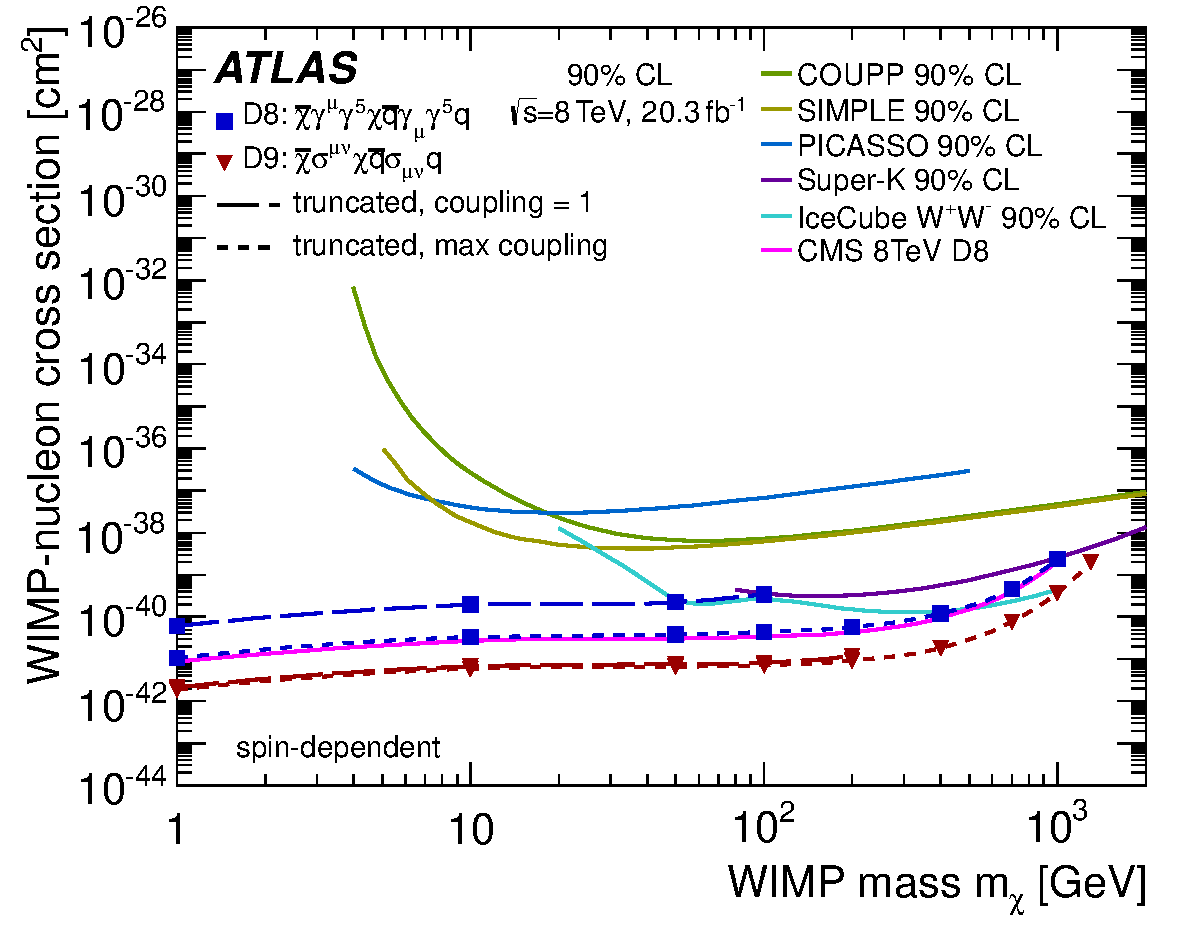
\includegraphics[width=0.35\textwidth]{figures/Monojet8TeV_EFT_SD}
%Can't have both so choose less controversial
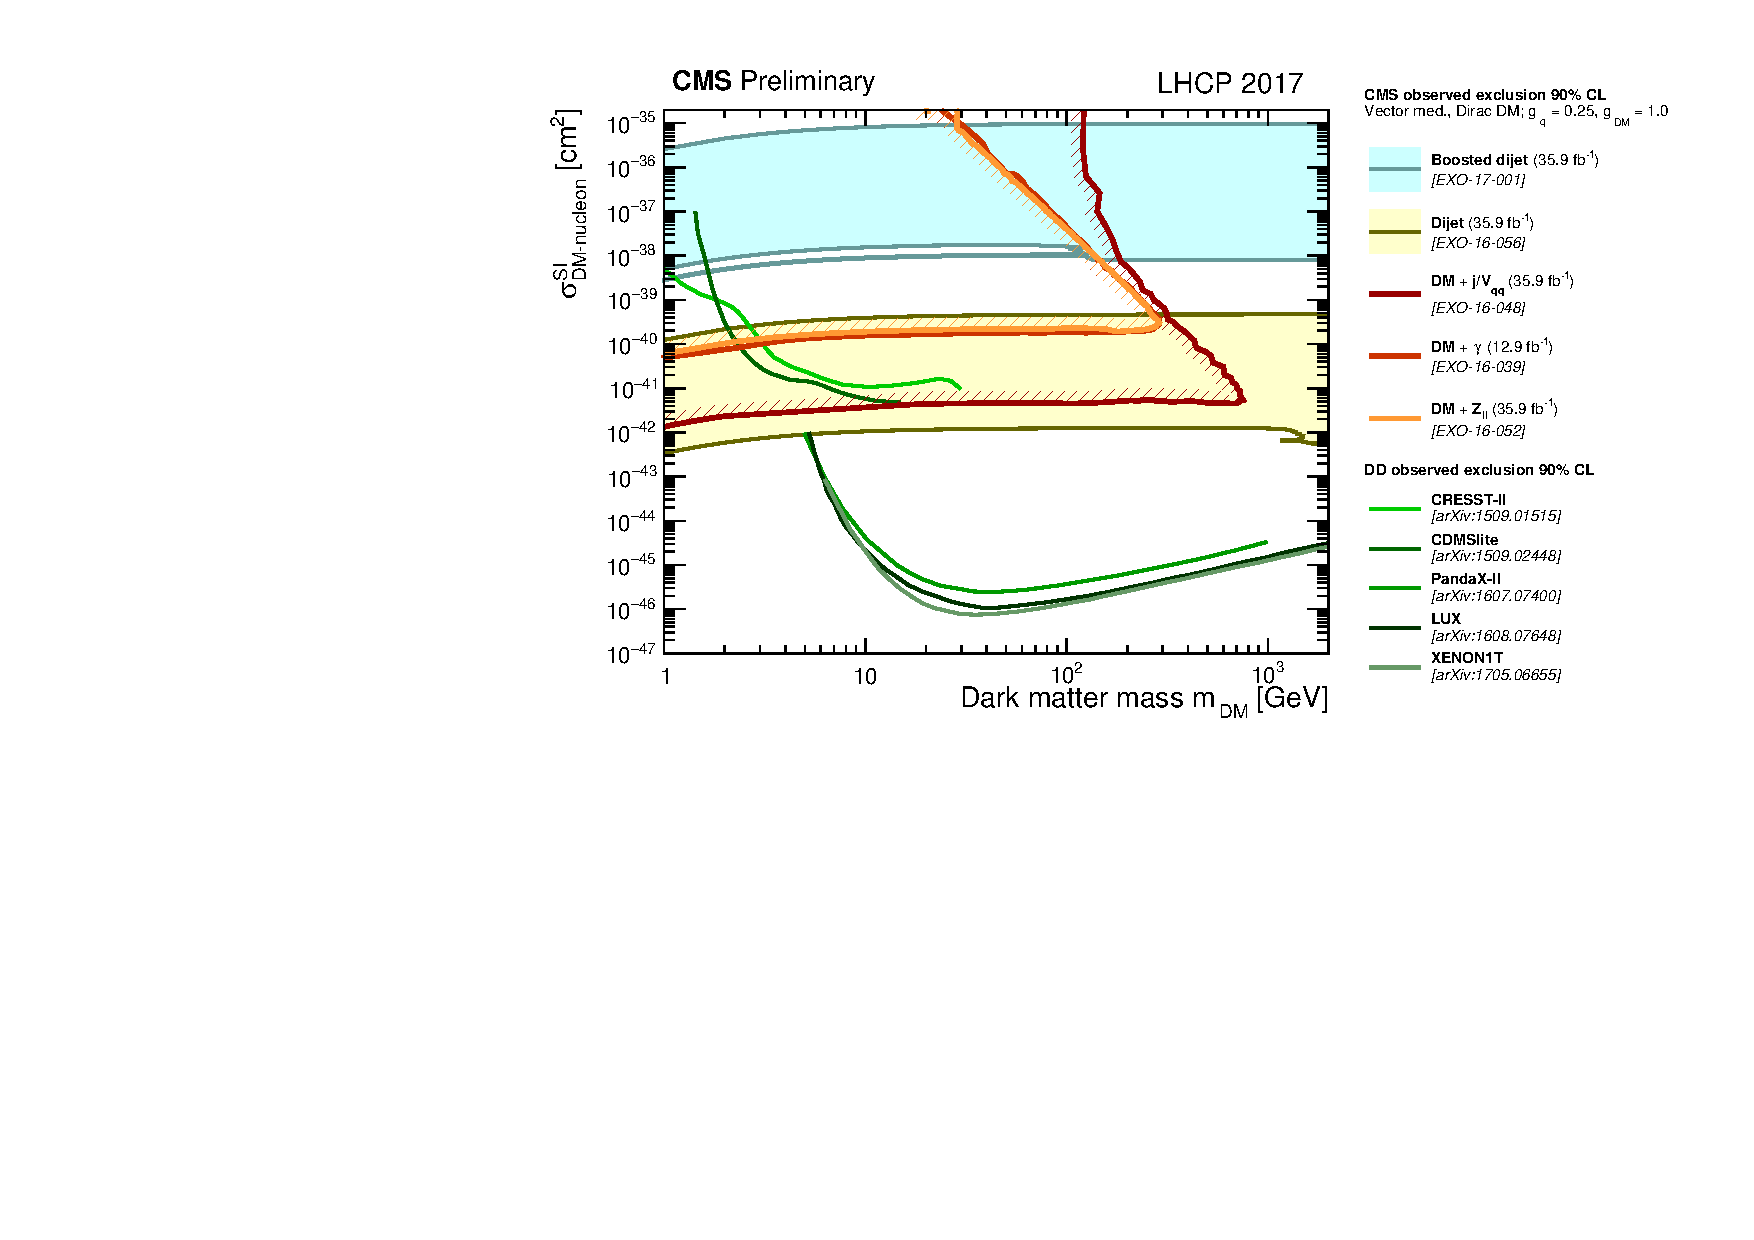
\includegraphics[width=0.9\textwidth]{figures/SI_CMSDD_Summary}
\caption{The 90\% CL CMS constraints in the \mdm-spin-independent DM-nucleon plane, for a vector mediator, Dirac DM and couplings gq = 0.25 and gDM = 1.0, compared with DD experiments. From~\cite{CMSSummary}.}
%We can update if something else comes out
\label{fig:SICMS}
\end{figure}
%Q: use SD? it will piss off more people but maybe we could make that point as well
%We could cite PDG review on spin-dependent vs spin-independent

With the adoption of simplified models of DM by LHC searches in Run-2~\cite{Abercrombie:2015wmb}, the
constraints and caveats of the comparisons between DD and ID have been made clearer, even though the comparisons themselves have become more model-specific and so far privileged vector and axial vector $s-$channel models with fixed coupling values. ATLAS and CMS follow a series of recommendations and well-defined procedure by the Dark Matter Working Group~\cite{Boveia:2016mrp}. LHC experimentalists and theorists have chosen to translate the collider results on visible mediator and invisible DM searches from the \mdm, \mmed plane to the DD and ID planes, so that all information on the results that are reinterpreted are available and all assumptions can be clearly spelled out. An example of such a comparison including the most recent LHC and DD results is shown in Fig.~\ref{fig:SICMSEFT}. In this kind of comparisons, it should be noted that the colliders limits do not include any constraint on the relic density, and that absolute exclusion of the different collider searches as well as their relative importance depend strongly on the benchmark scenario and its coupling. We also note that neither this procedure nor the benchmark models used are explicitly accounting for effects that may be important for mediators with masses below 100 GeV, such as interference and mixing with the X boson, quarkonia resonances and unitarity violation. 
%Could cite this for more consistent w/completion and ID: Jacques:2016dqz, but not sure what it adds, I prefer to talk about Linda's result
For reinterpretation of LHC results and their comparisons to DD and ID for scalar and pseudoscalar mediators, also in the context of 2HDM, see e.g.~\cite{Athron:2017kgt,Banerjee:2017wxi,Ipek:2014gua,Bell:2016ekl}.
%Proposals exist so that the plots should be truncated for cross-sections corresponding to a minimum mass.  
%Q: mention discussion from Landsberg? Would be nice. 
%https://indico.cern.ch/event/563066/contributions/2306614/attachments/1340042/2017991/DMWG-09-20-16.pdf
%Mention how low can one go in mdm - AB knows better here? 
%%DD/ID -> LHC
Recently, LHC results have also started to be utilized by DD collaboration for constraints of simplified models of DM, see e.g.\cite{PhysRevLett.118.251301,Balazs:2017hxh}. IceCube and other experiments have used constraints from a MSSM scan, see e.g.~\cite{Aartsen:2016zhm}.

The comparison of collider and ID results using simplified model benchmarks has received new attention since the publication of~\cite{Boveia:2016mrp}. In traditional comparisons, only one DM annihilation state at a time has been used for the comparison of collider and ID results (e.g. $b\bar{b}$, see for example~\cite{Agrawal:2014una}). The work in~\cite{Carpenter:2016thc} considers multiple final state fermions and interprets ID and LHC results in simplified models with $s-$ and $t-$channel mediators. 
%Would be nice to have a figure but probably too complicated to get as it's published

%Mention Gambit? I would rather describe it in the "SUSY fits" part

\subsection{Relic density}

